\documentclass[english]{article}
\usepackage[T1]{fontenc}
\usepackage[latin9]{inputenc}
\usepackage{geometry}
\geometry{verbose,tmargin=1.5in,bmargin=1.5in,lmargin=1.5in,rmargin=1.5in}
\usepackage{babel}
\usepackage{graphicx}
\usepackage{listings}
\usepackage{color}
\usepackage{hyperref}

\graphicspath{{../plots/}}

\lstdefinestyle{custompy}{
  belowcaptionskip=1\baselineskip,
  breaklines=true,
  frame=L,
  xleftmargin=\parindent,
  language=Python,
  showstringspaces=false,
  basicstyle=\footnotesize\ttfamily,
  keywordstyle=\bfseries\color{green},
  commentstyle=\itshape\color{red},
  identifierstyle=\color{black},
  stringstyle=\color{blue},
}


\lstset{escapechar=@,style=custompy}

\title{Random Sampling module for a drifting Maxwell-Juttner Distribution}
\author{Omkar H. Ramachandran}
\date{9 February 2018}


\begin{document}

\maketitle
\section{2D Contour plots of $f$}
\begin{figure}[h]
	\centering
	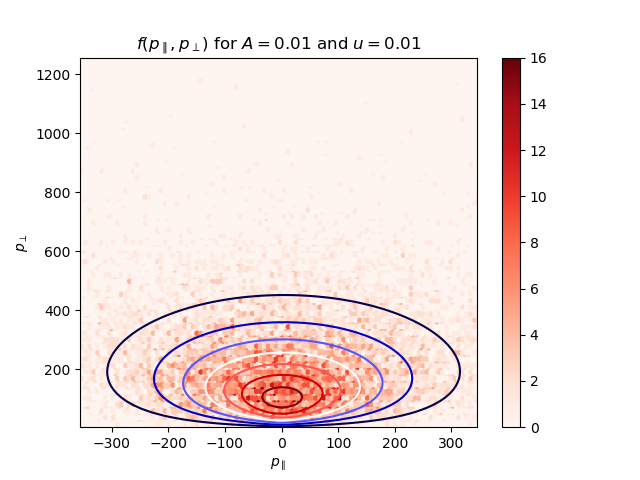
\includegraphics[width=0.33\textwidth]{plot_distribution_2D_u_0p01_A_0p01.png}
	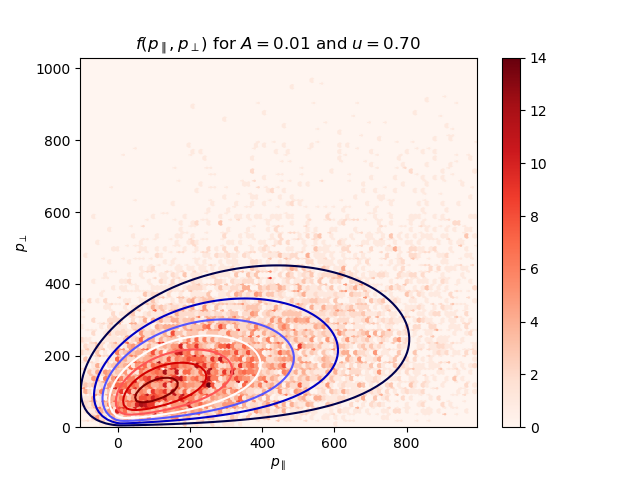
\includegraphics[width=0.33\textwidth]{plot_distribution_2D_u_0p7_A_0p01.png}
	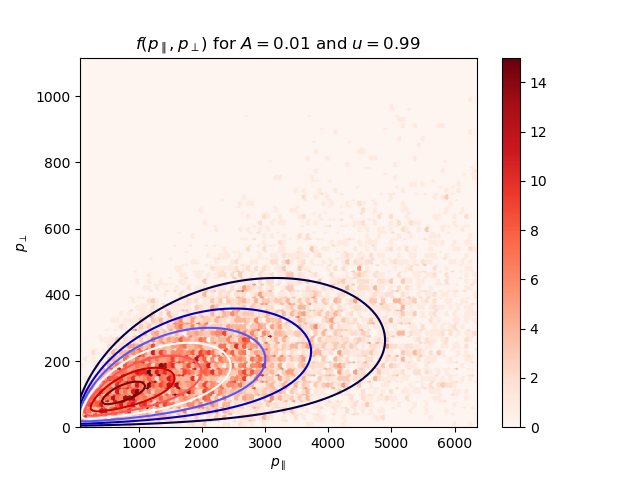
\includegraphics[width=0.32\textwidth]{plot_distribution_2D_u_0p99_A_0p01.png}

	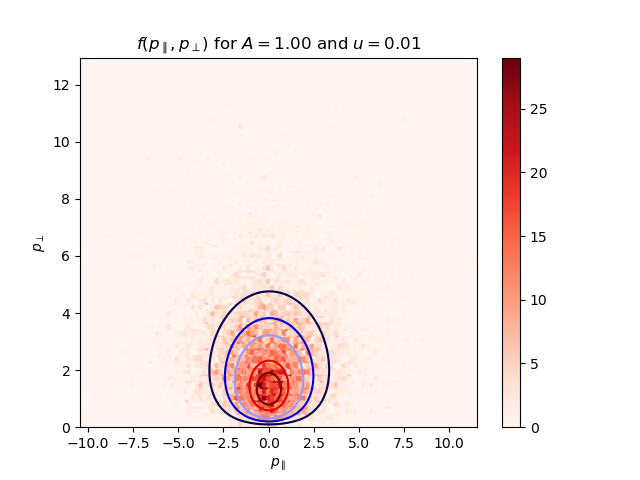
\includegraphics[width=0.33\textwidth]{plot_distribution_2D_u_0p01_A_1.png}
	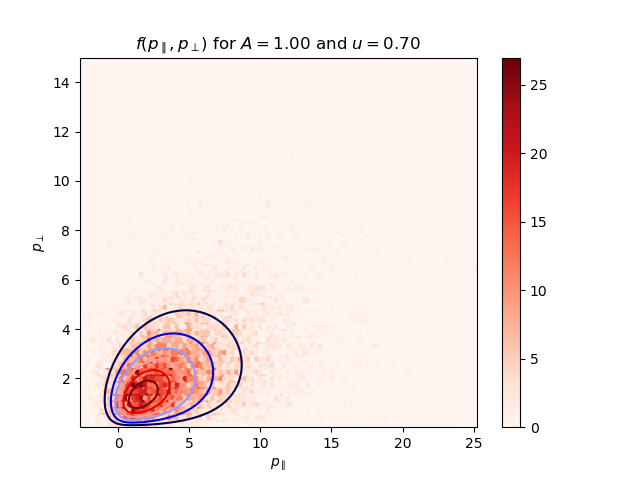
\includegraphics[width=0.33\textwidth]{plot_distribution_2D_u_0p7_A_1.png}
	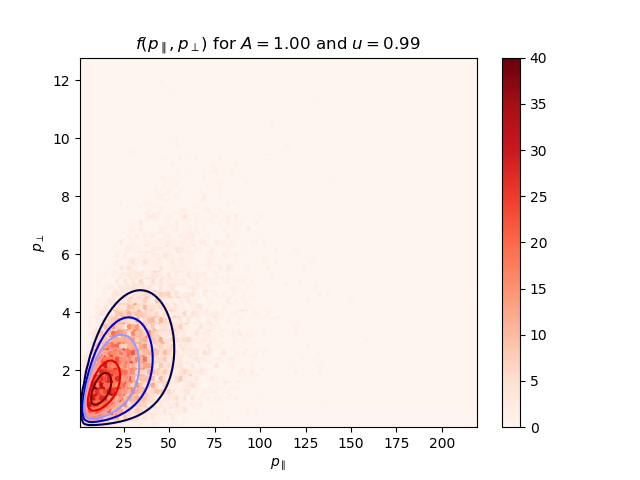
\includegraphics[width=0.32\textwidth]{plot_distribution_2D_u_0p99_A_1.png}
	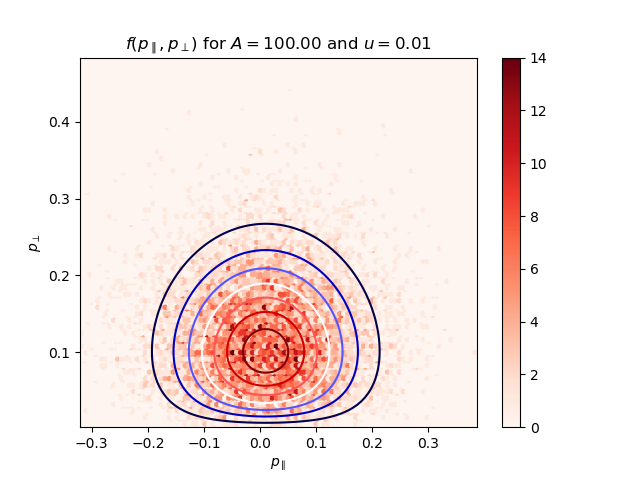
\includegraphics[width=0.33\textwidth]{plot_distribution_2D_u_0p01_A_100.png}
	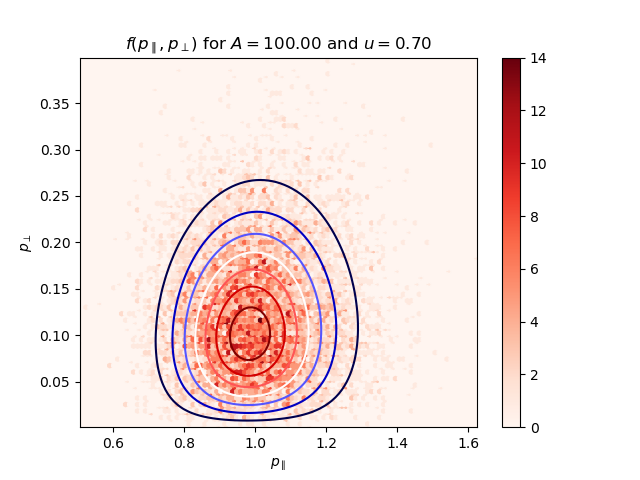
\includegraphics[width=0.33\textwidth]{plot_distribution_2D_u_0p7_A_100.png}
	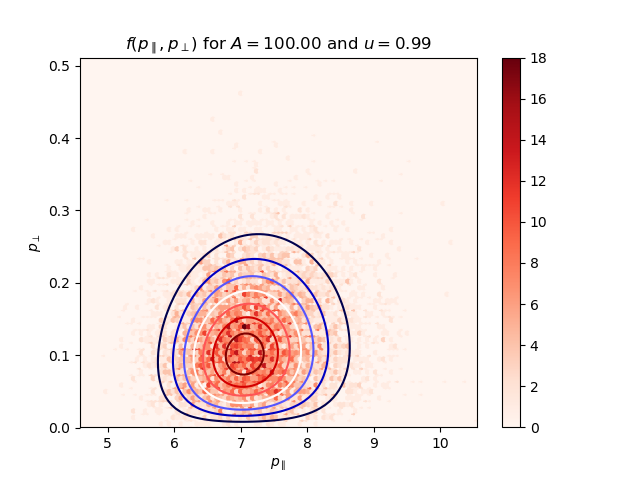
\includegraphics[width=0.32\textwidth]{plot_distribution_2D_u_0p99_A_100.png}
	\label{fig:high_A}
	\caption{Density plots of the generated histogram from $f$ with contours of the 
	analytically predicted districution overlaid. From each plot, we see that the 
	generated datapoints match the analytic function exactly}
\end{figure}

\end{document}
